\chapter{Evaluation}
\label{chap:evaluation}

We now evaluate our model through a series of microbenchmarks, system benchmarks and case studies.
First, we present the ARM and x86 hardware platforms used in addition to the cost of timer operations on those
platforms. Then we demonstrate the low performance overhead of our mechanisms using a set of 
microbenchmarks which measure the overheads of the MCS kernel versus a baseline, which is the \selfour
kernel, at development version 7.0.0 with some added experimental fastpaths for interrupt and signal
handling. Both branches have the same merge-base, \ie both branches divert from the master branch at
the same point. The exact revisions used are available online at:
\begin{description}
    \item[Baseline:] \url{https://github.com/pingerino/seL4/releases/tag/phd-baseline},
    \item[MCS:] \url{https://github.com/pingerino/seL4/releases/tag/phd-MCS}.
\end{description}

We then run several system benchmarks, first comparing a Redis~\citep{redis:url} 
implementation to baseline \selfour, Linux and NetBSD to show that our kernel is competitive.
We then demonstrate temporal
isolation between threads sharing the same CPU in two scenarios,
using Redis again, followed by ipbench~\citep{Wienand_Macpherson_04}. Finally, we show isolation in a
shared encryption server, and measure the cost of various timeout fault-handling policies. 

In addition, we evaluate two user-level scheduler implementations: one which implements a static
criticality switch, and a user-level \gls{EDF} implementation which we show is
competitive with an in-kernel \gls{EDF} scheduling from \litmus. Lastly, we use an \gls{IPC}
throughput benchmark to demonstrate low, multicore-scalability overhead, and we show 
how resource server threads can migrate between processing cores.

\section{Hardware}

% describe benchmark setup, details of each hardware platform
We run microbenchmarks on a variety of hardware to show the overheads of the model compared to
baseline \selfour. \Cref{t:evaluation-hardware} summarises the hardware platforms. \textsc{Sabre} is
the verified platform for \selfour, in addition to \text{x64}, which at the time of writing verification is
ongoing. Currently, the only platforms that support more than one core are \textsc{Sabre},
and \textsc{x64}.

Two of our platforms, \textsc{x64} and \textsc{Hikey} support both 32- and 64-bit execution modes.
We use both, referring to them as \textsc{ia32} and \textsc{Hikey32} when in 32-bit mode and
\textsc{x64} and \textsc{Hikey64} otherwise. All platforms have out-of-order execution, except
\textsc{Hikey}, which is in-order, and \textsc{KZM}, which has in order execution and out-of-order
from some operations (\eg stores).

Additionally, we use several load generators running Linux on an isolated network for 
benchmarks that require a network.

\begin{table}[t]
\begin{tabularx}{\textwidth}{Xlrrrrr}\toprule
    \emph{Platform}       & \emph{Microarch.} & \emph{Clock } & L1 & L2 & L3  & TLB  \\
    \emph{Arch}           & \emph{CPU}        & GHz           & (KiB) & (KiB) & (MiB) & (entries) \\\midrule
    \textsc{KZM} (32-bit) & ARM1136JF-S       & 1.0           & 16+16       & 128      & \no      & 32\\
    \small{ARMv6}                 & i.MX31            &               & 4$\times$        & 8$\times$         & \no      & 2$\times$  \\
    \rowcolor{gray!25}
    \textsc{Sabre} (32-bit) & Cortex-A9       & 1.0           & 32+32    & 1024     & \no      & 64\\
    \rowcolor{gray!25}
    \small{ARMv7}                    & i.MX6             &               & 4$\times$  & 16 $\times$  & \no & 2$\times$  \\
    \textsc{Hikey} (64-bit)  & Cortex-A53        & 1.2           & 32+32     & 512 & \no & 128         \\
    \small{ARMv8}                    & Kirin 620         &               & 4$\times$+2$\times$       & 16$\times$    & \no   & 4$\times$  \\
    \rowcolor{gray!25}
    \textsc{TX1}   (64-bit)  & Cortex-A57        & 1.9           &  32+48 & 2,048 & \no & 256          \\
    \rowcolor{gray!25}
    \small{ARMv8}                   & Jetson TX1  &                   & 2$\times$+3$\times$       & 16$\times$ & \no & 4$\times$ \\
    \textsc{x64}    (64-bit) & i7-4770           & 3.1           & 32+32 & 256 & 8 & 128,8 \\          
    \small{x86}                     & Haswell            &                 & 8$\times$ & 8$\times$ & 16$\times$ & 8$\times$ \\
    \bottomrule
\end{tabularx}
\caption[Hardware platform details.]{Hardware platform details, ``$\times$`` is associativity, and + indicates I-cache+D-cache.}
\label{t:evaluation-hardware}
\end{table}

\section{Overheads}

We first present a suite of microbenchmarks to evaluate any performance overheads against baseline
\selfour.
Because the kernel uses \emph{lazy switching} for the \gls{FPU}, where the \gls{FPU} context is only
switched if it is actively being used, we ensure \gls{FPU} context switching
is off. This is achieved by performing the required number of system calls 
without activating the \gls{FPU}. We present
overheads on IPC operations, signalling and interrupts, and finally scheduling. 

For each of the benchmarks in this section, we measure the cost of measurement, which is reading the
cycle counter on ARM platforms, and the \gls{TSC} on x86, and subtract the value obtained
from the final result.

\subsection{Timer}
\label{s:eval-timer}

Two of the main sources of overhead introduced by our model are related to the need to read and
reprogram the timer on non-fastpath kernel entries, and when performing a scheduling context switch.
We show the results of microbenchmarks of both of these operations in \Cref{t:evaluation-timer}, and
note the timer hardware used on the specific platform. 

\begin{table}[t]\centering
\rowcolors{2}{gray!25}{white}
\begin{tabularx}{\textwidth}{lXccc}\toprule
    \emph{Platform} & \emph{Timer} & \emph{Read time} & \emph{Set timeout} & \emph{Sum}
    \\\midrule
    \textsc{KZM}               & General purpose timer    & 83 (0)   & 203(0)  & 286   \\
    \textsc{Sabre}             & ARM MPCore global timer  & 23 (0)   & 36 (0)  & 59    \\
    \textsc{Hikey32/64}        & ARM generic timers       &  6 (0)   &  6 (0)  & 12    \\
    \textsc{TX1}               & ARM generic timers       &  8 (0)   &  1 (0)  & 9     \\
    \textsc{ia32}              & TSC deadline mode        & 12 (2.2) & 220 (1.0) & 232 \\
    \textsc{x64}               & TSC deadline mode        & 11 (2.3) & 217 (2.0) & 228 \\
    \bottomrule\hline
\end{tabularx}
\caption[Latency of timer operations.]{Latency of timer operations per platform in cycles. Standard deviations shown
in parentheses.}
\label{t:evaluation-timer}
\end{table}

For both microbenchmarks, we read the timestamp before and after the operation, and do this 102
times, discarding the first two results to prime the cache.  We take the difference of the cycle
counts, and subtract the cost of measuring the cycle counter itself. The results show the cost of
both operations separately, and then their sum, which is the total measured overhead introduced by timers on
scheduling context switch.

All platforms excluding \textsc{KZM} have a 64-bit timer available, making \textsc{KZM} the only
platform requiring timer overflow interrupts, which are not measured as \textsc{KZM} is a deprecated
platform provided for comparison with modern ARM versions.

\textsc{KZM} and \textsc{Sabre} both use memory-mapped timers, the 32-bit general purpose timer for
the former and 64-bit ARM global timer for the latter. \textsc{Sabre} has four cores and while the
timer device is shared, the timer registers are per-core, making access fast. 
Timer access on \textsc{Sabre} is significantly faster than the \textsc{KZM}. 

For all other ARM platforms, the ARM generic timers are available, which are accessed via the
coprocessor. The majority of new ARM platforms support the ARM generic timers. 

On \textsc{x64} we use the \gls{TSC} with \gls{TSC}-deadline
mode~\citep{Intel_64_IA-32:asdmspg_325384}, an architectural \gls{MSR} available since
Intel SandyBridge by which a local-APIC timer interrupt is triggered when the \gls{TSC} matches the
programmed value. 

\Cref{t:evaluation-timer} shows the instruction latency of each timer operation. In practice, especially
for \textsc{x64}, these operations are subject to pipeline parallelism and out-of-order execution, which
reduces the overhead.

Results on both architectures show that the overhead of a tickless kernel, which requires the timers
to be frequently read and reprogrammed, is tolerable on modern hardware. On ARM, timer costs have
reduced by an order of magnitude from ARMv6 through to ARMv8. 
\clearpage
\subsection{IPC performance}

\Gls{IPC} performance is a critical measure of the practicality and efficiency of a
microkernel~\citep{Liedtke_95}. We benchmark our \gls{IPC} operations against base system, \selfour,
which has an established efficient \gls{IPC} fastpath~\citep{Elphinstone_Heiser_13}. 

\subsubsection{Fastpath}

To evaluate IPC fastpath performance, we set up a client (the caller) and server (the callee) in different
address spaces. We take timestamps on either side of the IPC operation being benchmarked and record
the difference. This is done 16 times for each result value to prime the cache, then record the next
value. Results presented are for performing this a total of 16 times. Additionally, we measure the
overhead of system calls stubs in the same way and subtract this from the measurement, to obtain
only the kernel cost of the operation\footnote{The \gls{IPC} benchmarks already existed for
 \selfour, but we modify them to support the \gls{MCS} kernel as part of this thesis.}.
   The message sent is zero length, so neither the caller nor callee's \gls{IPC} buffer is accessed.

As discussed in \cref{p:impl-fastpath}, timer operations are avoided on the fastpath. However, we do
add significantly to the \call fastpath, by accessing two further objects (the scheduling context
and resume object) and two validation checks. In detail, the \call fastpath is altered as follows:

\begin{table}[t]\centering
    \rowcolors{2}{gray!25}{white}
    \begin{tabularx}{\textwidth}{Xrrrrrr}\toprule
        \emph{Platform}     
                                & \multicolumn{2}{c}{\emph{Baseline}}
                                & \multicolumn{2}{c}{\emph{MCS     }}
                                & \multicolumn{2}{c}{\emph{Overhead}} \\\midrule
    \ipcmicro{KZM}{kzm}{call-fastpath}
    \ipcmicro{Sabre}{sabre}{call-fastpath}
    \ipcmicro{Hikey32}{hikey32}{call-fastpath}
    \ipcmicro{Hikey64}{hikey64}{call-fastpath}
    \ipcmicro{TX1}{tx1}{call-fastpath}
    \ipcmicro{ia32}{ia32}{call-fastpath}
    \ipcmicro{x64}{haswell}{call-fastpath}
    \bottomrule
\end{tabularx}
\caption[Fastpath IPC overhead (\call)]{Time in cycles for the \call fastpath. Standard deviations shown in parentheses.}
\label{t:fastpath-ipc-micro-call}
\end{table}
\begin{table}[t]\centering
    \rowcolors{2}{gray!25}{white}
    \begin{tabularx}{\textwidth}{Xrrrrrr}\toprule
        \emph{Platform}      
                                & \multicolumn{2}{c}{\emph{Baseline}}
                                & \multicolumn{2}{c}{\emph{MCS     }}
                                & \multicolumn{2}{c}{\emph{Overhead}} \\\midrule
 
    \ipcmicro{KZM}{kzm}{reply-fastpath}
    \ipcmicro{Sabre}{sabre}{reply-fastpath}
    \ipcmicro{Hikey32}{hikey32}{reply-fastpath}
    \ipcmicro{Hikey64}{hikey64}{reply-fastpath}
    \ipcmicro{TX1}{tx1}{reply-fastpath}
    \ipcmicro{ia32}{ia32}{reply-fastpath}
    \ipcmicro{x64}{haswell}{reply-fastpath}
    \bottomrule
\end{tabularx}
\caption[Fastpath IPC overhead (\replyrecv)]{Time in cycles for the \replyrecv fastpath. Standard deviations shown in parentheses.}
\label{t:fastpath-ipc-micro-reply}
\end{table}

\begin{itemize}
\item We remove the reply capability lookup, so the sending \gls{TCB}'s \cnode is no
        longer accessed. 
\item We read the resume object pointer from the thread state, however the thread state is already accessed
    by the \call fastpath. 
\item We check that the resume object is valid. 
\item We read from and write to the resume object to push it onto the call stack.
\item We check the destination \gls{TCB} is passive.
\item We write scheduling context that is lent over the \call to link it to the receiver, and update
    the back pointer to the resume object.
\end{itemize}


\cref{t:fastpath-ipc-micro-call} shows the results.
Overheads on the \call fastpath are low, with the worst effected platform being
\textsc{KZM} with a 10\% overhead, which is the oldest platform with the smallest caches. On call,
\textsc{KZM} shows L1 data cache miss and 1 memory access, which is likely an unlucky cache-conflict. \textsc{Sabre} suffers a 7\% overhead, due to a \gls{TLB} miss likely
due to the relatively low associativity on Cortex-A9 \glspl{TLB}.  In general, as hardware becomes newer the
overhead is lower, with the exception of the \textsc{Hikey}, which is the only platform we use that has 
in-order execution. Additionally \textsc{Hikey} has a smaller L2 cache than the older \textsc{Sabre},
but a larger \gls{TLB} wit higher associativity.
We posit that for the Hikey, further hand optimisation of the fastpath would result in better
performance. The newest ARM hardware is the TX1, which only shows a 5\% overhead. x86 with its large
caches and highly optimised pipeline only incurs a 1\% overhead. For further detail on the
numbers read from the performance counters cited here, please see
\cref{appendix:fastpath-performance}.

The fastpath for \replyrecv has a higher impact, for two reasons: first, we add a new capability
lookup, being the resume object provided to receive, which must be looked up by the \replyrecv
fastpath. Although we remove of reply capability from the \gls{TCB}
\cnode, that \cnode is still accessed to validate the caller's root \cnode capability
and top-level page directory capability, so the cache-foot print is not reduced. Additionally, because
\gls{IPC} is now priority ordered, the fastpath must check if the callee's \gls{TCB} will be appended to the
endpoint queue. Otherwise, the fastpath is aborted for an ordered insert. 

As a result, the overheads shown in \cref{t:fastpath-ipc-micro-reply} for \replyrecv are generally higher
than \call, except for \textsc{Sabre}, which already suffered some \gls{TLB} misses on
the baseline kernel, again due to low \gls{TLB} associativity.
\clearpage

\subsubsection{Slowpath}
\label{eval:slowpath}

\begin{table}[t]\centering
    \rowcolors{2}{gray!25}{white}
    \begin{tabularx}{\textwidth}{Xlllllll}\toprule
        \input{data/generated/avg_slowpath_round_trip_passive.inc}
        \bottomrule
    \end{tabularx}
    \caption{Passive slowpath IPC overhead.}
    \label{t:slowpath-ipc-micro}
\end{table}
Now we evaluate the \gls{IPC} slowpath, for both active and passive threads. Unlike the fastpath, the slowpath
generally does not fit into the cache. Consequently precise measurements like those done for the
fastpath show erratic results with high standard deviations on our hardware. Instead, we run average
benchmarks for the slowpath, where for 110 runs, we measure the time taken for 10,000 IPC pairs
(\call, \replyrecv) and divide by 10,000 to get a result.
In order to hit the slowpath we make the message length 10 words, which exceeds
the fastpath condition that the message should fit into registers.

We run the benchmark for both active and passive threads, which shows the overhead of changing a
scheduling context versus not. \cref{t:slowpath-ipc-micro} shows the results for the passive
slowpath and \cref{t:slowpath-ipc-micro-active} for active, where the top row in the table is 
the baseline number, the second row is the overhead when
comparing the number of cycles taken for the benchmark. Every other row shows difference in value of the 
listed performance counter between baseline and MCS. We do not show standard deviations, however
they are measured and are very small (either 0 or a few percent of the mean). 

Passive slowpath overhead, as shown in \cref{t:slowpath-ipc-micro} is not small;
this is due to the fact that the seL4 scheduler has far more
functionality than previously, increasing the code size, and the cache foot print is higher, given
that the resume object and scheduling context must be accessed in addition to the \glspl{TCB} of the
caller and callee. Looking at ARM platforms, the overhead reduces drastically as hardware becomes
more modern: for the most part, this means that the caches are bigger, and timer access costs are
smaller. This is with the exception of the \textsc{Hikey} platform, with has an in-order
execution pipeline and a smaller L2 cache than the \textsc{Sabre}. We suspect that the overheads could be reduced on Hikey with more careful hand
optimisation. 64-bit Hikey has nearly half the excess instructions when compared to 32-bit, and far
50\% less memory accesses, resulting in far less overhead on \textsc{Hikey64} than \textsc{Hikey32}.
\textsc{Sabre} suffers from the low-associativity of its \gls{TLB} with misses in both the instruction and
data TLBs. On the x86 platform, both \textsc{ia32} and \textsc{x64} show the same overhead in terms
of ratio, both due to the increase in instructions.

Another factor that complicates the slowpath is the compiler. We use GCC version 5.5.0 with optimisation
level O2 for all benchmarks, with the \code{mtune} parameter set as appropriate. All of the kernel
code is pre-processed and concatenated into to single file with the \code{whole-program} attribute
set which allows for greater compiler optimisations. However, the level of optimisation for a
specific platform, especially ARM platforms, is not know and contributes to the variance between
platforms, and between arm versions.

Additionally, it should be noted that the slowpath is avoided in most cases, as long IPC is discouraged in
favour of establishing shared memory protocols to transfer large amounts of data. The majority of
fastpath checks make sure the thread being switched to is valid and runnable. Only two cases hit the
slowpath frequently: if a medium priority thread has woken, and is higher priority than the
\gls{IPC} target, and if the target is active, not passive. 
Additionally, many improvements can be made to the \gls{IPC} slowpath to improve
performance, but it has not been examined extensively.

\begin{table}[t]\centering
    \rowcolors{2}{gray!25}{white}
    \begin{tabularx}{\textwidth}{Xlllllll}\toprule
        \input{data/generated/avg_slowpath_round_trip.inc}
        \bottomrule
    \end{tabularx}
\caption{Active slowpath IPC overhead.}
\label{t:slowpath-ipc-micro-active}
\end{table}


\cref{t:slowpath-ipc-micro-active} shows results for the active slowpath, and has higher overheads
again. In this case, we change scheduling
contexts, so not only does another object (the second \gls{SCO}) need to be accessed, but the timer
needs to be reprogrammed, and sporadic replenishment logic applied. \textsc{TX1} and
\textsc{Hikey64} have the lowest overhead, although the overhead looks to be ameliorated by lucky
data placement with a reduction in L1 D-cache misses on both platforms. The vast majority of
overhead comes from far more instructions executed, and on platforms with small caches or
low-associativity, the increase in cache footprint.  


\subsection{Faults}

\begin{table}[t]\centering
    \rowcolors{2}{gray!25}{white}
    \begin{tabularx}{\textwidth}{Xllllll}\toprule
\input{data/generated/avg_fault_round_trip_passive.inc}
    \bottomrule
\end{tabularx}
\caption[Passive fault IPC overhead.]{Passive fault IPC overhead baseline \selfour compared with MCS. All
values excluding the first two rows shows the baseline performance counter value subtracted
from the MCS performance counter value.}
\label{t:slowpath-fault-micro}
\end{table}

\begin{table}[t]\centering
    \rowcolors{2}{gray!25}{white}
    \begin{tabularx}{\textwidth}{Xllllll}\toprule
\input{data/generated/avg_fault_round_trip.inc}
    \bottomrule
\end{tabularx}
\caption[Active fault IPC overhead.]{Active fault IPC overhead baseline \selfour compared with MCS. All
values excluding the first two rows shows the baseline performance counter value subtracted
from the MCS performance counter value.}
\label{t:slowpath-fault-micro-passive}
\end{table}

Recall that fault handling in \selfour occurs via an \gls{IPC}, simulated by the kernel, to a fault
endpoint, which a fault handling-thread can wait upon for messages (\cref{api:faults}). 

To measure the fault-handling cost, we run two threads in the same address space: a fault handler
and a faulting thread, with the same priority. We trigger a fault by executing an undefined instruction in a loop on the faulting thread's
side. The fault handler then increments the instruction pointer past the undefined
instruction, and the benchmark continues.  As this is also a slowpath, we use the same method as
above, and measure the amount of time it takes for 10,000 faults then divide the result. We do this
for 110 runs, abandoning the first 10, to calculate the standard deviation and average. 

We measure both active and passive fault handling, and the results, shown in
\cref{t:slowpath-fault-micro}, are similar to slowpath
\gls{IPC}, being slower for active, and improving as cache-size and timer operation cost reduces. 
Note that although there is currently no fastpath for fault handling, it is merely a matter of
engineering effort to add one should this become a performance issue. 

We do not show results for the \textsc{KZM} platform, as it is ARMv6 and the performance monitor
unit, including the cycle counter, cannot be read from user mode. As a result we use the
undefined instruction to read the cycle counter efficiently on this platform, 
so the fault benchmark does not work.

\subsection{Signalling and interrupts}

\begin{table}[t]\centering
\begin{tabular}{cl r@{~}l r@{~}l r@{~}r}\toprule
\emph{Platform}           & \multicolumn{1}{c}{\emph{Operation}}
                                & \multicolumn{2}{c}{\emph{Base}}
                                & \multicolumn{2}{c}{\emph{MCS}}
                                & \multicolumn{2}{c}{\emph{Overhead}} \\
%    \irqmicro{KZM}{kzm}
%    \irqmicro{Sabre}{sabre}
%    \irqmicro{Hikey32}{hikey32}
%    \irqmicro{Hikey64}{hikey64}
%    \irqmicro{TX1}{tx1}
%    \irqmicro{ia32}{ia32}
%    \irqmicro{x64}{haswell}
    \bottomrule
\end{tabular}
\caption[Fastpath IRQ and Signal overhead.]{Fastpath IRQ and signal overhead in cycles, baseline
    \selfour versus MCS. Standard deviations shown in parentheses.}
\label{t:micro-irq}
\end{table}

As noted in the previous section, mainly engineering effort is required to add new fastpaths. For
this reason, we add two new (non-verified) experimental fastpaths to the baseline and MCS kernels: one for interrupt
delivery, and the other for signalling a low-priority thread, which we now examine.

We measure interrupt latency using two threads, one spinning in a loop
updating a volatile cycle counter, the other, higher priority thread
waiting for an interrupt. On delivery, the handler thread determines the
interrupt latency by subtracting the
looped timestamp from the current time. \cref{t:micro-irq} shows the results. 
The overhead is higher here as we must switch scheduling
contexts, which requires reprogramming the timer, however the scheduler is by-passed as the switch
is to a higher priority thread. \textsc{KZM} shows the  highest overhead, where once again we
exceed the small cache. The \textsc{Hikey} pays for its in-order execution pipeline, which could be
improved with further profiling of the fastpath. The \textsc{TX1} shows the least impact, with only
a 5\% increase on the interrupt fastpath.

\code{signal()}, on the other hand shows little overhead as it does not alter the
scheduling context or access to the timer device.  In this benchmark, a high priority thread signals
a low priority thread, a common operation for interrupt service routines. As \cref{t:micro-irq}
shows, in 
cases where slowpath performance is a issue, further fastpaths can be added to avoid accessing the
timer, in the case where older hardware is required.

\subsection{Scheduling}

\begin{table}[t]\centering
    \rowcolors{2}{gray!25}{white}
    \begin{tabularx}{\textwidth}{Xlllllll}\toprule
\input{data/generated/schedule_process_average.inc}
\end{tabularx}
\caption[Slowpath scheduler costs.]{Slowpath yield and scheduler costs in cycles, baseline \selfour 
versus MCS. Standard deviations shown in parentheses.}
\label{t:micro-schedule}
\end{table}

\begin{table}[t]\centering
    \rowcolors{2}{gray!25}{white}
    \begin{tabularx}{\textwidth}{Xlllllll}\toprule
\input{data/generated/Average_seL4_Yield_no_thread_switch.inc}
\end{tabularx}
\caption[Yield to self scheduler costs.]{Yield to self costs.Slowpath yield and scheduler costs in cycles, baseline \selfour 
versus MCS. Standard deviations shown in parentheses.}
\label{t:micro-schedule}
\end{table}

In our final microbenchmark we look at the cost of the scheduler, and the \yield system call. 

The \code{schedule} benchmark measures the cost of a signal to a higher priority thread, which forces 
a reschedule operation and does not avoid picking a new thread from the scheduler, in addition to
all other slowpath overheads. Like the other slowpath benchmarks, we take the average of 10,000
runs. 
The scheduler is by definition a slowpath activity, as it is completely avoided on the fastpath, and
much of the slowpath, by the lazy scheduling mechanism (\cref{sec:sel4-scheduler-opt}).
\cref{t:micro-schedule} shows that scheduling cost increases noticeably, however note that \selfour IPC,
particularly scheduler-context donation (and its predecessor, the
undisciplined timeslice donation), is designed to minimise the need for
invoking the scheduler, therefore this increase is unlikely to have
a noticeable effect in practice. 

We also measure the average cost for the current thread to \yield to itself. The overhead is large 
as \yield is nearly a completely different system call: previously \yield was incomplete, and would simply
dequeue and enqueue the current thread from the scheduling queues, before returning to user level.
\yield in the new model charges the remaining budget in the head replenishment to the thread, and
triggers a timer reprogram. Although semantically similar for round robin threads, \yield does a lot
more, hence the drastic overheads shown in \cref{t:micro-schedule}.

\subsection{Full system benchmark}
\label{s:evaluation-redis-overhead}

To demonstrate the impact of the overheads in a real system scenario, 
we measure the performance of the Redis key value store~\citep{redis:url} using 
\gls{YCSB}~\citep{Cooper_STRS_10} on baseline and MCS \selfour, and compare this
against Linux, the Rump unikernel~\citep{Kantee_Cormack_14} and 
NetBSD~\citep*{NetBSD:url} all on the \textsc{x64} machine. Note that the Rump unikernel only
currently supports x86 platforms, consequently experiments requiring Rump are only carried out on
the \textsc{x64} platform. 

For \selfour, we use a single-core Rump library OS~\citep{Kantee_Cormack_14} to provide 
NetBSD network drivers at user level, by leveraging an existing port of this infrastructure
to \selfour~\citep{McLeod:be}.
The system consists of Redis/Rump running on three active \selfour threads: 
two for servicing interrupts (network, timer) and one for Rump, as shown in
\cref{f:redis-arch}. Interrupt threads run at the highest priority,
followed by Redis and a low-priority idle thread (not shown) for measuring CPU utilisation;
this setup forces frequent invocations of the scheduler and interrupt path.

 \begin{figure}[ht]
    \centering
    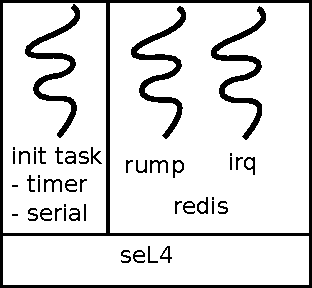
\includegraphics{redis-arch}
    \caption[System architecture of Redis benchmark.]{System architecture of the Redis / \gls{YCSB} benchmark on \selfour, 
        Linux, NetBSD and Rump unikernel.}
    \label{f:redis-arch}
\end{figure}

\cref{t:redis} shows the achieved throughput of Redis+Rump
running \gls{BMK}, and Redis on the seL4 baseline and as well as the MCS
branch, plus Linux and NetBSD (7.0.2) for comparison. \cref{f:redis-arch} shows the \selfour set up,
compared with the architecture of Redis on Linux, NetBSD and \gls{BMK}. 

\cref{t:redis} indicates the interrupt handling method used, as there is no single method supported
across all four scenarios. \gls{BMK} only supports the legacy
\gls{PIC},
while NetBSD only supports \glspl{MSI}. Linux and seL4 both support the
\gls{APIC}.

The utilisation figures show that the system is fully loaded, except
in the Linux case, where there is a small amount of idle time. The
cost per operation (utilisation over throughput) is best on Linux, a
result of its highly optimised drivers and network stack. Our
bare-metal and \selfour-based setups use Rump's NetBSD drivers, and
actually performance within a few percent of native NetBSD. This
indicates that the MCS model comes with low overhead.

\begin{table}[t]\centering
      \rowcolors{3}{}{gray!25}
      \begin{tabularx}{\textwidth}{Xrrrrr}\toprule
          \emph{System}   & \emph{IRQ} & \emph{Throughput} & \emph{Utilisation} & \emph{Cost} & \emph{Latency} \\
                          &            & (k ops/s)         & (\%)               & per op.     & (ms)            \\
        \midrule

      \input{data/ycsb-redis.inc}
      \bottomrule
    \end{tabularx}
    \caption[Results of Redis throughput benchmark.]{Throughput (k\,ops/s) achieved by Redis using the YCSB
      workload A with 2 clients.  Latency is the average Read and Update,
      standard deviations in parentheses and omitted where less than the least
      significant digit shown.}
    \label{t:redis}
\end{table}

\section{Temporal Isolation}

We have demonstrated our model has little overhead and is competitive with existing monolithic
kernels. Now we evaluate temporal isolation properties, between processes and in a shared-server
scenario. 
In addition, we evaluate and demonstrate different
techniques to restore server state after a timeout exception.

% Show isolation between processes using different scheduling contexts
\subsection{Process isolation} 

We evaluate process isolation, where processes do not share resources, indirectly via network
throughput and network latency in two separate benchmarks. 
\subsubsection{Network throughput}

First, we demonstrate our isolation properties with the Redis architecture described in
\Cref{s:evaluation-redis-overhead}, with an additional, high-priority active CPU-hog thread
competing for \gls{CPU} time.  All scheduling contexts in the system are configured with a
5\,ms period. We use the budget of the CPU-hog to control the amount of time left over
for the server configuration. \autoref{f:redis} shows the throughput
achieved by the YCSB-A workload as a function of the available CPU
bandwidth (i.e \ the complement of the bandwidth granted to the CPU-hog
thread). All data points are the average of three benchmark runs.

\begin{figure}[h]
  \centering
  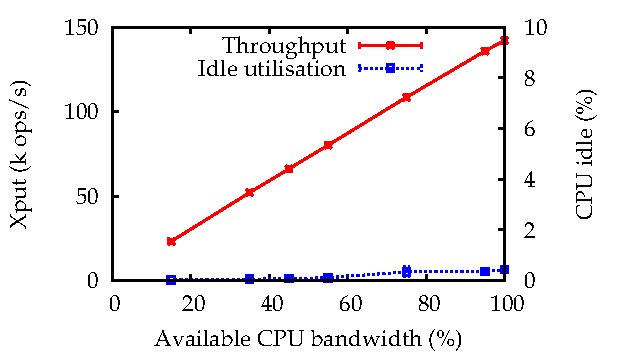
\includegraphics{redis}
  \caption[Results of Redis isolation benchmark.]{Throughput of Redis YCSB workload A and idle time versus available bandwidth.}
  \label{f:redis}
\end{figure}

The graph shows that the server is CPU limited (as indicated by very low idle time)
and consequently throughput scales linearly with available CPU
bandwidth.

\subsubsection{Network latency}

Second, we evaluate process isolation via network latency in a system shown in \cref{f:ipbench-arch}. 
The system consists of a single-core of a Linux \gls{VM} which runs at a high priority with a
constrained budget and a \gls{UDP} echo server running at a lower priority,
representing a lower-rate \textsc{high} thread. We
measure the average  and maximum UDP latency reported by the
ipbench~\citep{Wienand_Macpherson_04} latency test.

\begin{figure}[h]
    \centering
    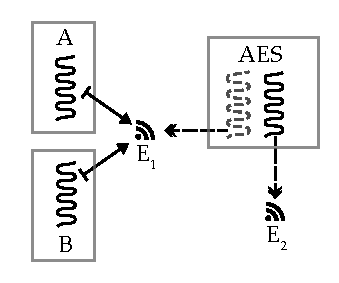
\includegraphics{ipbench-arch}
    \caption{System architecture of ipbench benchmark.}
    \label{f:ipbench-arch}
\end{figure}


Specifically, the Linux VM interacts with timer (PIT) and serial device drivers implemented as
passive servers outside the \gls{VM}; all three components are at a high priority. In the Linux server we
run a program (\code{yes > /dev/null}) which consumes all available
CPU bandwidth.  The UDP echo server, completely isolated from the Linux instance during the
benchmark, but sharing the
serial driver, runs at a low priority with its own HPET timer
driver.

Two client machines run ipbench daemons to send packets to the UDP-echo server on the target machine
(\textsc{x64}). The control machine, one of the load generators, runs ipbench with a \gls{UDP} socket at 10\,Mbps over a 1\,Gb/s Ethernet connection with 100-byte packets. The Linux VM has a 10\,ms period and we vary the
budget between 1\,ms and 9\,ms.
We represent the zero-budget case by an unconstrained Linux that is not running any user code.
Any time not consumed by Linux is available to UDP echo for processing
10,000 packets per second, or 100 packets in the time left over from
each of Linux's 10\,ms period.

\autoref{f:ipbench} shows the average and maximum \gls{UDP} latencies for
ten runs at each budget setting. We can see that the maximum latencies
follow exactly the budget of the Linux server (black line) up to 9\,ms. Only
when Linux has a full budget (10\,ms), and thus able to monopolise the
processor, does the UDP server miss its deadlines, resulting in a
latency spike.  This result shows that our sporadic server implementation is effective in bounding
interference of a high-priority process.

\begin{figure}[h]
  \centering
  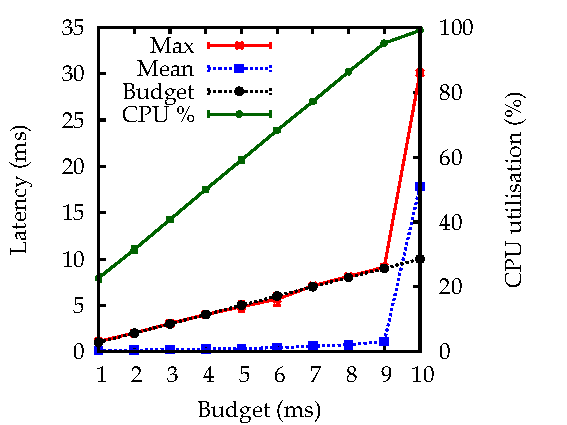
\includegraphics{ipbench}
  \caption[Results of ipbench isolation benchmark.]{Average and maximum latency of UDP packets with
  a CPU-hog VM running a high priority with a 10\,ms budget.}
  \label{f:ipbench}
\end{figure}

% Show isolation in a shared server
\subsection{Server isolation} 
\label{s:server-isolation}

To demonstrate temporal isolation in a shared server, we use a case study of an encryption service
using \gls{AES} to encrypt client data. We measure both the overhead of different
recovery techniques, and the throughput achieved when two clients constantly run out of budget in the server. 
We port an existing, open-source \gls{AES} implementation to a shared server running on \selfour, and run
benchmarks on both \textsc{x86} and \textsc{Sabre}.

\Cref{f:aes-arch} shows the architecture of the case study. Both clients $A$ and $B$ are single
 threaded and exist in separate address spaces to the server. The server has two threads, a passive
 thread for serving requests on the client's scheduling context and an active thread which handles
 timeout exceptions for the server. The server and timeout exception handler share the same virtual
 memory and capability spaces.

\begin{figure}
\centering
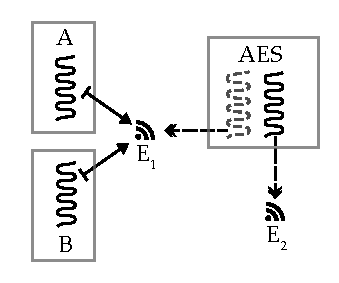
\includegraphics{aes-arch}
\caption[Architecture of the AES case study.]{Architecture of the \gls{AES} case study. Client $A$ and $B$ make \gls{IPC} requests over
endpoint $E_{1}$ of passive $AES$ which has an active timeout fault handling thread waiting for
fault \gls{IPC} messages on endpoint $E_{2}$.}
\label{f:aes-arch}
\end{figure}

The server itself runs the AES-256 algorithm with a block size of 16~bytes. The server alternates between two
buffers, using an atomic swap, of which one always contains consistent state, the other is
dirty during processing. When a timeout fault occurs, only the dirty buffer is lost due to
inconsistency. Both clients request 4\,MiB of data to be encrypted, provided by a shared buffer
between client and server, and have a budget insufficient to
complete the request. When the server is running on the client's scheduling context and the budget
expires, a timeout exception, which is a fault IPC message from the kernel, is delivered to the timeout
handler. 

\subsection{Timeout handling techniques}

If a client's scheduling context is depleted while the server is servicing the request, a timeout fault
is raised and sent to the timeout handler.  The appropriate protocol for handling such faults
depends ultimately on the requirements of the system.  Consequently, we implement and evaluate four
different timeout fault handling techniques: \emph{rollback}, \emph{error}, \emph{emergency} and
\emph{extend}. 

While each technique is evaluated separately, combinations of such techniques could be used for
different clients, depending on their requirements. For example, trusted clients may get special
treatment. Note that in all cases of blocking IPC, clients must trust the server as discussed in
\cref{s:locking}. Additionally, although our experiment places 
the timeout fault handler in the server's address
space, this is not necessary: for approaches that require access to scheduling contexts and
scheduling control capabilities, the timeout handler may be placed in a scheduling server's address
space, separate from the server itself.

\subsubsection{Rollback}

Rollback restores the server to the last known consistent state recorded. In the case of non-thread
safe servers, this may require rolling back an entire request. However, algorithms like \gls{AES}
which can easily be batched can make progress. The process for rollback is as follows:

\begin{enumerate}\label{e:rollback}
    \item A timeout fault is received by timeout handler, $T$ over $E_{2}$.
    \item $T$ constructs a reply message to the client from the last clean state, and sends this 
        message to the client by invoking the resume capability that the server has used for that client. 
        Because the resume object tracks the donation, the client's scheduling context is returned.
    \item $T$ then restores the server, $S$, to a known state (restoring registers,
        stack frames and any global state). $S$ is restored to the point before it made its
        last system call, usually an \nbsendrecv, which it used to indicate to the initialiser that
        $S$ should be made passive, as part of the passive server initialisation protocol presented
        in \cref{sec:impl-passive-servers}.
    \item Now the server must return to blocking on the IPC endpoint, $E_{1}$. $T$ binds a
        scheduling context to $S$ and waits for a message. 
    \item Now the $S$ runs from its checkpoint, repeating the \nbsendrecv, signalling to $T$ that it
        can now be converted to passive once more and blocking on $E_{1}$. 
    \item $T$ wakes and converts the server back to passive.
    \item Finally, $T$ blocks on $E_{2}$, ready for further timeout faults.
\end{enumerate}

The rollback technique requires the server and timeout handler to both have access to the reply
object that the server is using, and the server's \gls{TCB}, meaning the timeout handler must be
trusted by the server. In our example the server and timeout handler run at the same priority, in
all cases both must run at higher priorities than the clients, to allow the timeout handler to
reinitialise the server in the correct order, and to implement the \gls{IPCP}. 

Once the budget of the faulting client is replenished, it can then continue the request based on the
content of the reply message sent by the timeout handler. Clients are guaranteed progress as long as
their budget is sufficient to complete a single batch of data.

If rollback is not suitable, the server can be similarly reset to the initial state and an error
returned to the client. However, this does not guarantee progress for clients with insufficient
budgets.

\subsubsection{Kill}

In cases of non-preemptible servers, potentially due to a lack of thread safety, one option is to
kill client threads. Such a scenario would stop untrusted misbehaving clients from constantly
monopolising server time.  We implement an example were the timeout handler has access to client \gls{TCB}
capabilities and simply calls suspend, however the server could also switch to a new reply object
and leave the client blocked forever, without access to any of the clients capabilities. 

The process for suspending the client is the same as that for \Cref{e:rollback} but for two aspects;
the server state does not need to be altered by the timeout handler as the server always 
restores to the same place, instead of replying to the client it is suspended.

\subsubsection{Emergency}

Another technique gives the server a one-off emergency budget to finish the client request, after
which the exception handler resets the server to being passive. This could be used in low
criticality \gls{SRT}
scenarios where isolation is desired but transient overruns are expected.
An example emergency protocol follows:

\begin{enumerate}\label{e:emergency}
    \item A timeout fault is received by timeout handler, $T$ over $E_{2}$.
    \item $T$ unbinds the client scheduling context from $S$.
    \item $T$ binds a new scheduling context to $S$, which acts as an emergency budget.
    \item $T$ then replies to the timeout fault, resuming $S$.
    \item Now $T$ enqueues itself on $E_{1}$, such that when the server finishes the blocked request,
        $T$, being a higher priority, is served next.
    \item $S$ completes the request and replies to the client.
    \item $S$ receives the request from $T$, and replies immediate as it is an empty request.
    \item $T$ wakes, and converts the server back to passive.
    \item Finally $T$ blocks on $E_{2}$, ready for further timeout faults.
\end{enumerate}

This case requires the timeout handler to have access to clients' scheduling contexts, in order to
unbind them from the server. 

\subsubsection{Extend}

The final technique is to simply increase the client's budget on each timeout, which requires the
timeout fault handler to have access to the client's scheduling contexts.
This could be deployed in \gls{SRT} systems or for specific threads with unknown budgets up to a limit. 

\begin{enumerate}\label{e:extend}
    \item A timeout fault is received by timeout handler, $T$ over $E_{2}$.
    \item $T$ extends the client's budget by configuring scheduling context.
    \item $T$ replies to the fault message, which resumes $S$.
\end{enumerate}

%\newpage
\begin{table}[t!]\centering
\begin{tabular}{cllrrrr}\toprule
\emph{Platform} & \emph{Operation} & \emph{Cache} & \emph{Min} &
                          \emph{Max} & \emph{Mean} &
                          \multicolumn{1}{c}{\boldmath \(\sigma\)} \\\midrule
                          \multirow{8}{*}{\textsc{x64}}
                          \input{data/generated/haswell-aes.inc}
                          \midrule
                          \multirow{8}{*}{\textsc{Sabre}} 
                          \input{data/generated/sabre-aes.inc} 
                          \midrule
                          \multirow{8}{*}{\textsc{Hikey64}} 
                          \input{data/generated/hikey64-aes.inc} 
                          \midrule
                          \multirow{8}{*}{\textsc{TX1}} 
                          \input{data/generated/tx1-aes.inc} 
                          \bottomrule
\end{tabular}
\caption[Cost of timeout handler operations.]{Cost of timeout handler operations in \(\mu\)s, as measured
  by timeout exception handler. \(\sigma\) is the standard deviation.}
\label{t:rollback}
\end{table}


\subsection{Results}

We measure the pure handling overhead in each case, from when the timeout handler wakes up to when
it blocks again.  Given the small amount of rollback state, this measures the baseline overhead. For
schedulability analysis, the actual cost of the rollback would have to be added, in addition to the
duration of the timeout fault IPC. 
 
We run each benchmark with hot caches (primed by some warm-up
iterations)  as well as cold (flushed) caches and measure the 
latency of timeout handling, from the time the handler wakes up
until it replies to the server.

\autoref{t:rollback} shows the results. The maximum
colD-cache cost, which is relevant for schedulability analysis, differs by a factor of 3--4 between
the different recovery scenarios, indicating that all are about equally feasible.  Approaches that
restart the server and send \glspl{IPC} messages on its behalf (rollback, reply) are the most
expensive as they must restore the server state from a checkpoint and follow the passive server
initialisation protocol (recall \cref{sec:impl-passive-servers}). 

\subsection{Rollback isolation}

\begin{figure}[t]
  \centering
  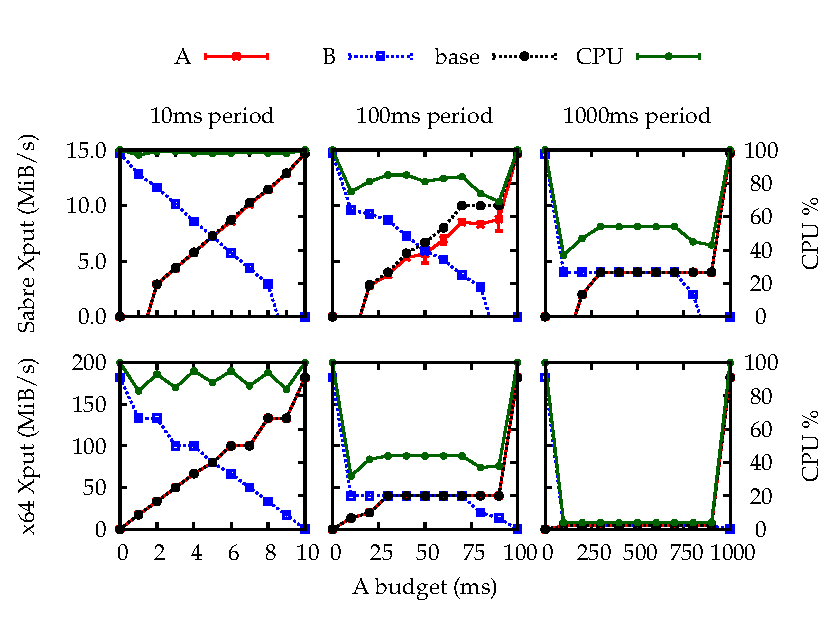
\includegraphics{aes-shared}
  \caption[Results of AES server isolation benchmark.]{Throughput for clients A and B of a passive AES server processing 10 requests of 4\,MiB of data with
      limited budgets on the \textsc{x64} (top row) and \textsc{Sabre} (bottom row) platforms. The two clients' budgets
      add up to the period, which is varied between graphs (10, 100, 1000\,ms). Clients sleep when
      they process each 4\,MiB, until the next period, except when their budgets are full. Each data point is the average of 10 runs, error bars show the standard deviation.}
  \label{f:aes}
\end{figure}

We next demonstrate temporal isolation in the server by using the rollback
technique and measuring the time taken to encrypt 10 requests of 4\,MiB of
data. \autoref{f:aes} shows the result with both clients having the same
period, which we vary between 10\,ms and 1000\,ms.
In each graph we vary the clients' budgets between 0 and the
period. The extreme ends are special, as one of the clients has a full
budget and keeps invoking the server without ever getting rolled back,
thus monopolising the processor. In all other cases, each client
processes at most 4\,MiB of data per period, and either succeeds (if
the budget is sufficient) or is rolled back after processing less than 4\,MiB.

The results show that in the CPU-limited cases (left graphs)
we have the expected near perfect proportionality between throughput and
budget (with slight wiggles due to the rollbacks), showing isolation between clients. In the cases where there is headspace (centre of the right
graphs), both clients achieve their desired throughput.

\section{Practicality}

Fundamental to the microkernel philosophy is keeping policy out of the
kernel as much as possible, and instead providing general mechanisms
that allow the implementation of arbitrary policies
\citep{Heiser_Elphinstone_16}.  As on the face of it, our
fixed-priority-based model seems to violate this principle,  we
demonstrate that the model is general enough to support the efficient
implementation of alternate policies at user level. Specifically, we
implement two user-level schedulers: first, a static mixed criticality
scheduler~\citep{Baruah_BD_11}, which we also compare to an in-kernel
implementation, and an \gls{EDF} scheduler, which we compare to \litmus.

\subsection{Criticality}

\begin{figure}[t]
  \centering
  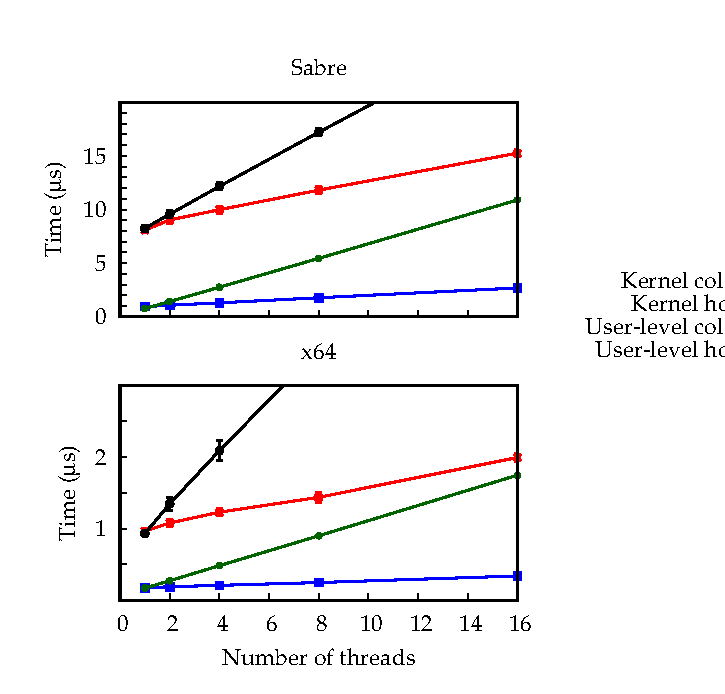
\includegraphics[width=\textwidth]{mode-switch-all}
  \caption[Kernel vs. user-level criticality switch.]{Cost of switching the priority of $n$ threads in kernel and user level, with hot
      and cold caches, on \textsc{x64} (top-left), \textsc{TX1} (top-right), \textsc{Hikey64}
      (bottom-left) and \textsc{Sabre} (bottom-right). All data points are the average of 100 runs,
                  with very small standard deviations.}
  \label{f:mode-switch}
\end{figure}


Static, mixed-criticality, fixed-priority schedulers are based on \emph{mode
switches}, which effectively mean altering the priority of threads in bulk:
critical threads that may be of low rate are bumped to higher than their
low-criticality counter parts, to ensure deadlines are met in exceptional
circumstances. 

We implement a kernel mechanism for changing thread priorities in bulk,
and compare with a user-level approach which simply changes the priority of threads
one at a time. In our prototype implementation, the kernel tracks all threads of specific
criticalities and boosts their priority on a criticality switch. However, given threads are kept in per-priority queues, each thread must be removed and reinserted into a new queue, so either way the complexity of the mode-switch is $O(n)$. 

\begin{table}[t]\centering
    \rowcolors{2}{gray!25}{}
    \begin{tabular}{lrrr}\toprule
        \emph{Platform}     & \emph{Kernel cold ($\mu$s)} & \emph{User-level cold ($\mu$s)} & \emph{Diff $\mu$s} \\\midrule
        \textsc{x64}    & $\leq2$ & $\leq4$ & \textasciitilde2 \\
        \textsc{TX1}    & $\leq4$ & $\leq8$ & \textasciitilde4 \\
        \textsc{Hikey64}    & $\leq18$ & $\leq30$ & \textasciitilde12 \\
        \textsc{Sabre}    & $\leq12$ & $\leq22$ & \textasciitilde10 \\
        \bottomrule
\end{tabular}
\caption[Comparison of kernel and user-level priority switches]{Comparison of cold, in-kernel
priority switch to cold, user-level priority switch.}
\label{t:cold-prio-switch}
\end{table}


\autoref{f:mode-switch} shows the results measured with a primed cache (hot) and flushed cache (cold).
As the graph shows, switching is linear in the number of threads being boosted, in both kernel and
user-level implementations.
\Cref{t:cold-prio-switch} compares the results of cold, in-kernel switching to user-level in roughly
absolute terms. \textsc{Hikey64} is the slowest at 30\,\(\mu\)s with eight threads to switch,
due to the smaller L2 cache and
in-order execution, however all platforms show roughly the same factor of two increase when
comparing kernel and user-level cold-cache results.
However, most systems will not have more than a few high-criticality threads, and deadlines for critical control loops in
cyber-physical systems tend to be in the tens of milliseconds, we
conclude that criticality can be implemented at user-level, in line with standard microkernel philosophy.

The higher cost from user-level operation results from  multiple
switches between kernel and user mode, and the repeated
thread-capability look-ups. It could be significantly reduced if seL4
had a way to batch system calls, but to date we have seen no compelling use cases for this.

As a second criticality-switch benchmark, we ported three processor intensive 
benchmarks from the MiBench~\citep{Guthaus_REAMB_01} to act as workloads. 
We use \textsc{susan}, which performs image recognition, \textsc{jpeg}, which does image
encoding/decoding, and \textsc{mad}, which plays an MP3 file.
Each benchmark runs in its own Rump process
with an in-memory file system, and shares a timer and serial server.
 We chose these specific
benchmarks as they were the easiest to adapt as described below, and use them as workloads,
rather than for comparing systems, so there is no issue of bias from sub-setting.

We alter the benchmarks to run periodically in multiple stages. To obtain
execution times long enough, some benchmarks iterate a fixed number of times per
stage. Each benchmark process executes its workload and then waits for the next period to start.
Deadlines are implicit: if a periodic job finishes before the start of the next period, it is
considered successful, otherwise the deadline is missed.

We run the benchmarks on both the user-level and in-kernel implementations of static mixed criticality, with 10 runs of each.

\begin{table}[t]
    \centering
    \begin{tabular}{lcccccclcl}\toprule
        \emph{Application} & \emph{T} & \emph{L} & \emph{\(L_S\)} & \emph{C} & \emph{U} & \emph{j} &
        & \emph{m}  & \\\midrule
        \input{data/generated/mode_switch.inc}
        \bottomrule
    \end{tabular}
    \caption[Results of criticality switch benchmark.]{Results of criticality switch benchmark for each
        stage, where the  criticality \(L_S\) is raised each stage. \(T\) =
        period, \textit{C} = worst observed execution time (ms),
      \textit{U} = allowed utilisation (budget/period),
      \textit{m} = deadline misses, \textit{j} = jobs completed. We record 52 (0.1), 86 (15.2)
      and 100 (0.0)\% CPU
utilisation for each stage respectively. Standard deviations are shown in parentheses. Bold values
show the difference between the user-level scheduler and kernel. }
    \label{t:modeswitch}
\end{table}


Results are shown in \autoref{t:modeswitch}. For both schedulers (kernel versus user-level), 
the results are nearly exactly the same. Bold numbers indicate a difference between the kernel and
user-level scheduler, with only the lowest-criticality thread affected by the criticality switch, with an additional missed deadline due to
perturbations in run time due to the slightly slower user-level scheduler.
For stage one, the entire workload is schedulable and
there are no deadline misses. For stage two, the workload is not
schedulable, and the criticality switch boosts the priorities of
\textsc{susan} and \textsc{jpeg}, such that they meet
their deadlines, but
\textsc{mad} does not. In the final stage, only the most critical task
meets all deadlines.
This shows that it is sufficient to implement criticality at user-level, and our mechanisms operate as intended.

\subsection{User-level EDF}\label{s:edf-impl}

\begin{listing}
\inputminted{c}{code/edf.c}
\caption{Pseudocode for the EDF scheduler.}
\label{list:edf}
\end{listing}

We implement the EDF scheduler as an active server with active
clients which run at an \selfour priority below the user-level scheduler.
The scheduler waits on an endpoint on which it receives messages from
its clients and the timer, as shown in \cref{list:edf}.

Each client has a period, representing its relative deadline, and a full reservation (equal to the period). Clients
either notify the scheduler of completion by an IPC
message, or else create a timeout exception on preemption, which is also received by the
scheduler. Either is an indication that the next thread should be scheduled.

\begin{figure}[t]
\centering
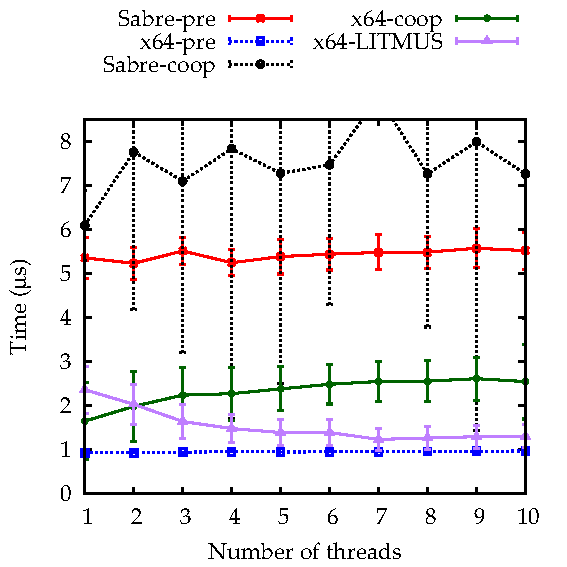
\includegraphics{edf}
\caption[Results of \selfour user-level EDF versus \litmus.]{Execution time of \selfour user-mode EDF scheduler compared to
         kernel scheduler in \textsc{x64} \litmus.}
\label{f:edf}
\end{figure}


We use the \emph{randfixedsum}~\citep{Emberson_SD_10} algorithm to
generate deadlines between 10 and 1000\,ms for a certain number of threads.
A set of threads runs until 100
scheduling decisions have been recorded. We repeat this 10 times,
resulting in 1,000 scheduler runs for each data point.

We measure the scheduler latency by recording the timestamp when each client thread, and an idle
thread, detects a
context switch and processing the difference in timestamp pairs offline. We run two schedulers:
\emph{pre}-empt where threads never yield and must incur a timeout exception, and \emph{coop}, where
threads use IPC to yield to the scheduler. The latter invokes the user-level timer
driver more often as the release queue is nearly always full, which involves more kernel invocations
to acknowledge the IRQ, in addition to reprogramming the timer.

We compare our latencies to those of
LITMUS$^{RT}$~\citep{Calandrino_LBDA_06}, a widely-used real-time scheduling
framework for developing real-time schedulers and locking protocols. 
As it is  embedded in Linux, LITMUS$^{RT}$ is not aimed at high-assurance systems.

We use Feather-Trace~\citep{Brandenburg_Anderson_07} to gather data.
We use the C-EDF scheduler, which is a partitioned (per-core) EDF scheduler, on a single
core. We use the same parameters and thread sets, running each set for 10\,s. 
The measured overhead considers the in-kernel scheduler, context-switch and user-level code to return to
the user.

\autoref{f:edf} shows that our preemptive user-level EDF scheduler implementation is
actually faster than the in-kernel EDF scheduler from LITMUS$^{RT}$, and
that the cost of implementing scheduling policy at user level is of
the same order as the in-kernel default scheduler. In other words,
implementing different policies on top of the base scheduler is quite feasible.
\section{Multiprocessor benchmarks}

We run two multicore benchmarks, the first evaluating multicore throughput of the MCS kernel versus the
baseline kernel, the second based on our shared server \gls{AES} case study to demonstrate the
multicore model. 

We run multiprocessor benchmarks on two of our platforms, \textsc{Sabre} and \textsc{x64}. Both 
are symmetric multiprocessors with four cores. 

\begin{figure}[t] 
    \centering
    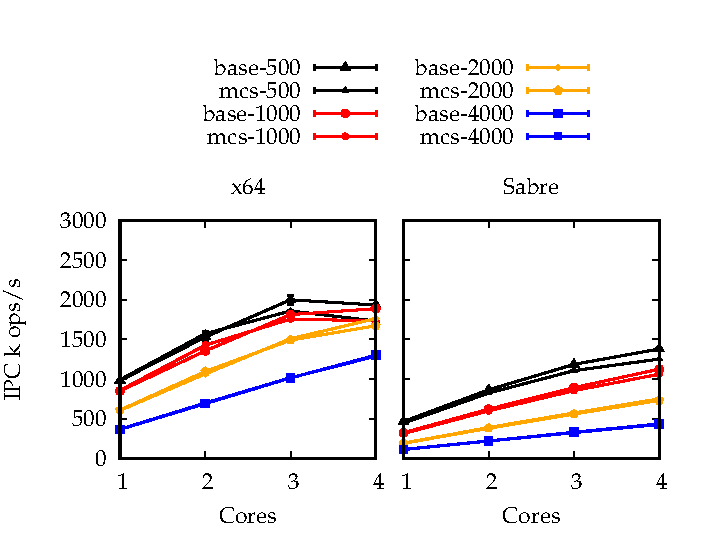
\includegraphics{smp}
    \caption[Results of the multicore IPC throughput benchmark.]{Results of the multicore IPC throughput benchmark, baseline \selfour vs MCS. 
        Each series is named \textit{name-N}, where \textit{name} is \textit{base} and \textit{mcs} for 
        the baseline and MCS kernel respectively, and \textit{N} is the upper
        bound on the number of cycles between each IPC for that series.}
    \label{f:evaluation-smp}
\end{figure}

\subsection{Throughput}

We run a multicore throughput benchmark to show that our MCS model
avoids introducing scalability problems on multiple cores compared to the baseline kernel.
We modify the
existing multicore IPC throughput benchmark for \selfour to run on the MCS kernel. 
At time of writing, only \textsc{x64} and \textsc{sabre} have \selfour multiprocessor support, 
consequently these are the platforms used for the benchmark.

The existing multicore benchmark measures IPC throughput of a client and server, both 
pinned to the same processor, sending fastpath, 0-length IPC messages via \call
and \replyrecv. One pair of client and server is set up per core. Both threads are
the same priority and the messages are 0 length. Each thread spins for a random amount
with an upper bound \textit{N} between each subsequent IPC. As \textit{N} increases so does
IPC throughput, as fewer calls are made.

We modify the benchmark such that each server thread is passive on the MCS kernel.
Results are displayed in \Cref{f:evaluation-smp} and show a minor impact on IPC throughput
for low values of \textit{N}. Scalability is not impacted on \textsc{sabre}, but is on \textsc{x64},
with the curve flattening slightly more aggressively on the MCS kernel
due to the fastpath overhead. The low overhead is expected as the MCS model only introduces extra 
per-core state, with no extra shared state between cores. The slight scalability impact is
due to a higher cache-footprint of the IPC fastpath. 
\clearpage
\subsection{Shared server}

\begin{figure}[t] 
    \centering
    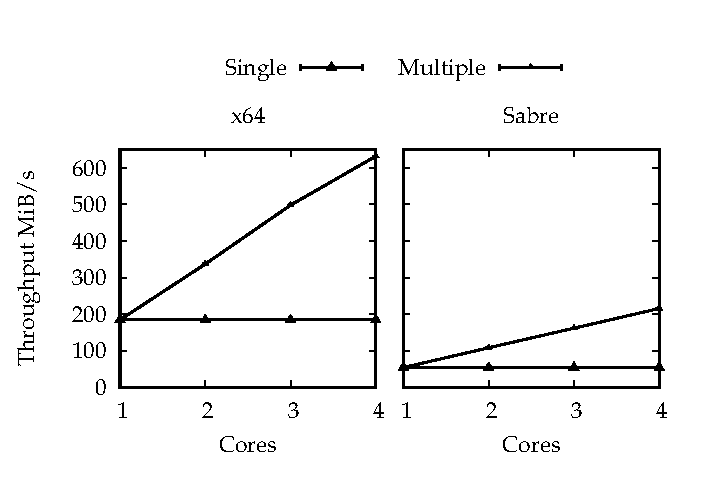
\includegraphics{smp_aes}
    \caption[Results of the AES shared server multicore case study.]{Results of the AES shared server multicore case study. \emph{Single} shows results for a 
        passive server thread migrating between cores to service clients, while \emph{Multiple} has one
        passive server thread per core. For both series, the number of clients is equal to the number of
        cores and each client requests 1MiB of data encrypted. }
    \label{f:evaluation-smp-aes}
\end{figure}

We adapt our \gls{AES} case study (\cref{s:server-isolation}) to demonstrate how our MCS model 
applies to multiprocessors. The AES server is configured without a timeout fault handler, and
we run two variants. 

\begin{description}
    \item[Single:] the AES server has a single passive thread, which waits on a single endpoint
        and migrates to the core of the active client over IPC, effectively serialising access to the server.
        Consequently, \cref{f:evaluation-smp-aes} shows there is no gain in throughput when further cores are
        added. 
    \item[Multiple:] the AES server has one passive thread per core, and an endpoint is set up for
        each core, demonstrating a parallel server. Due to the absence of bottlenecks in the stateless 
        AES server, this results in near perfect scalability.
\end{description}

\section{Summary}

All in all, we have demonstrated via micro- and macro- benchmarks that our overheads are
reasonable given the speed of the baseline kernel and the extent of the provided
functionality. 

Through two system benchmarks and one shared-server benchmark, we have shown
that our approach guarantees processor isolation and that threads cannot exceed
their budget allocation via their scheduling context. Additionally, we have
shown that isolation can be achieved in a shared server via a timeout-fault
handler, and implemented several alternatives for handling such faults,
demonstrating the feasibility of the model. 

Policy freedom is maintained despite providing fixed-priority scheduling in the kernel, as the
mechanisms are sufficient to implement low-overhead, user-level schedulers, 
as demonstrated through the static, mixed-criticality and EDF scheduler
implementations. 

Finally, we have demonstrated that the model works for multiprocessors,
incurring no great scalability penalty over baseline \selfour, 
and show how passive servers migrate across cores on \gls{IPC}.
